
%%%%%%%%%%%%%%%%%%%%%%%%%%%%%%%%%%%%%%%%%%%%%%%%%%%%%%%%%%%%%%%%%%%%%
\savegeometry{beamergeo}
\begin{emptyframe}
%\begin{frame}[plain,label=TitlePage]
\begin{center}
\textcolor{Blue}{Electronic and structural instabilities} \\
\vspace{0.5em}
{\footnotesize F. M. Grosche} \\
{\footnotesize \em Cavendish Laboratory, Cambridge} \\
\vspace{0.1em}
\end{center}
\vspace{0.0em}
\centerline{ 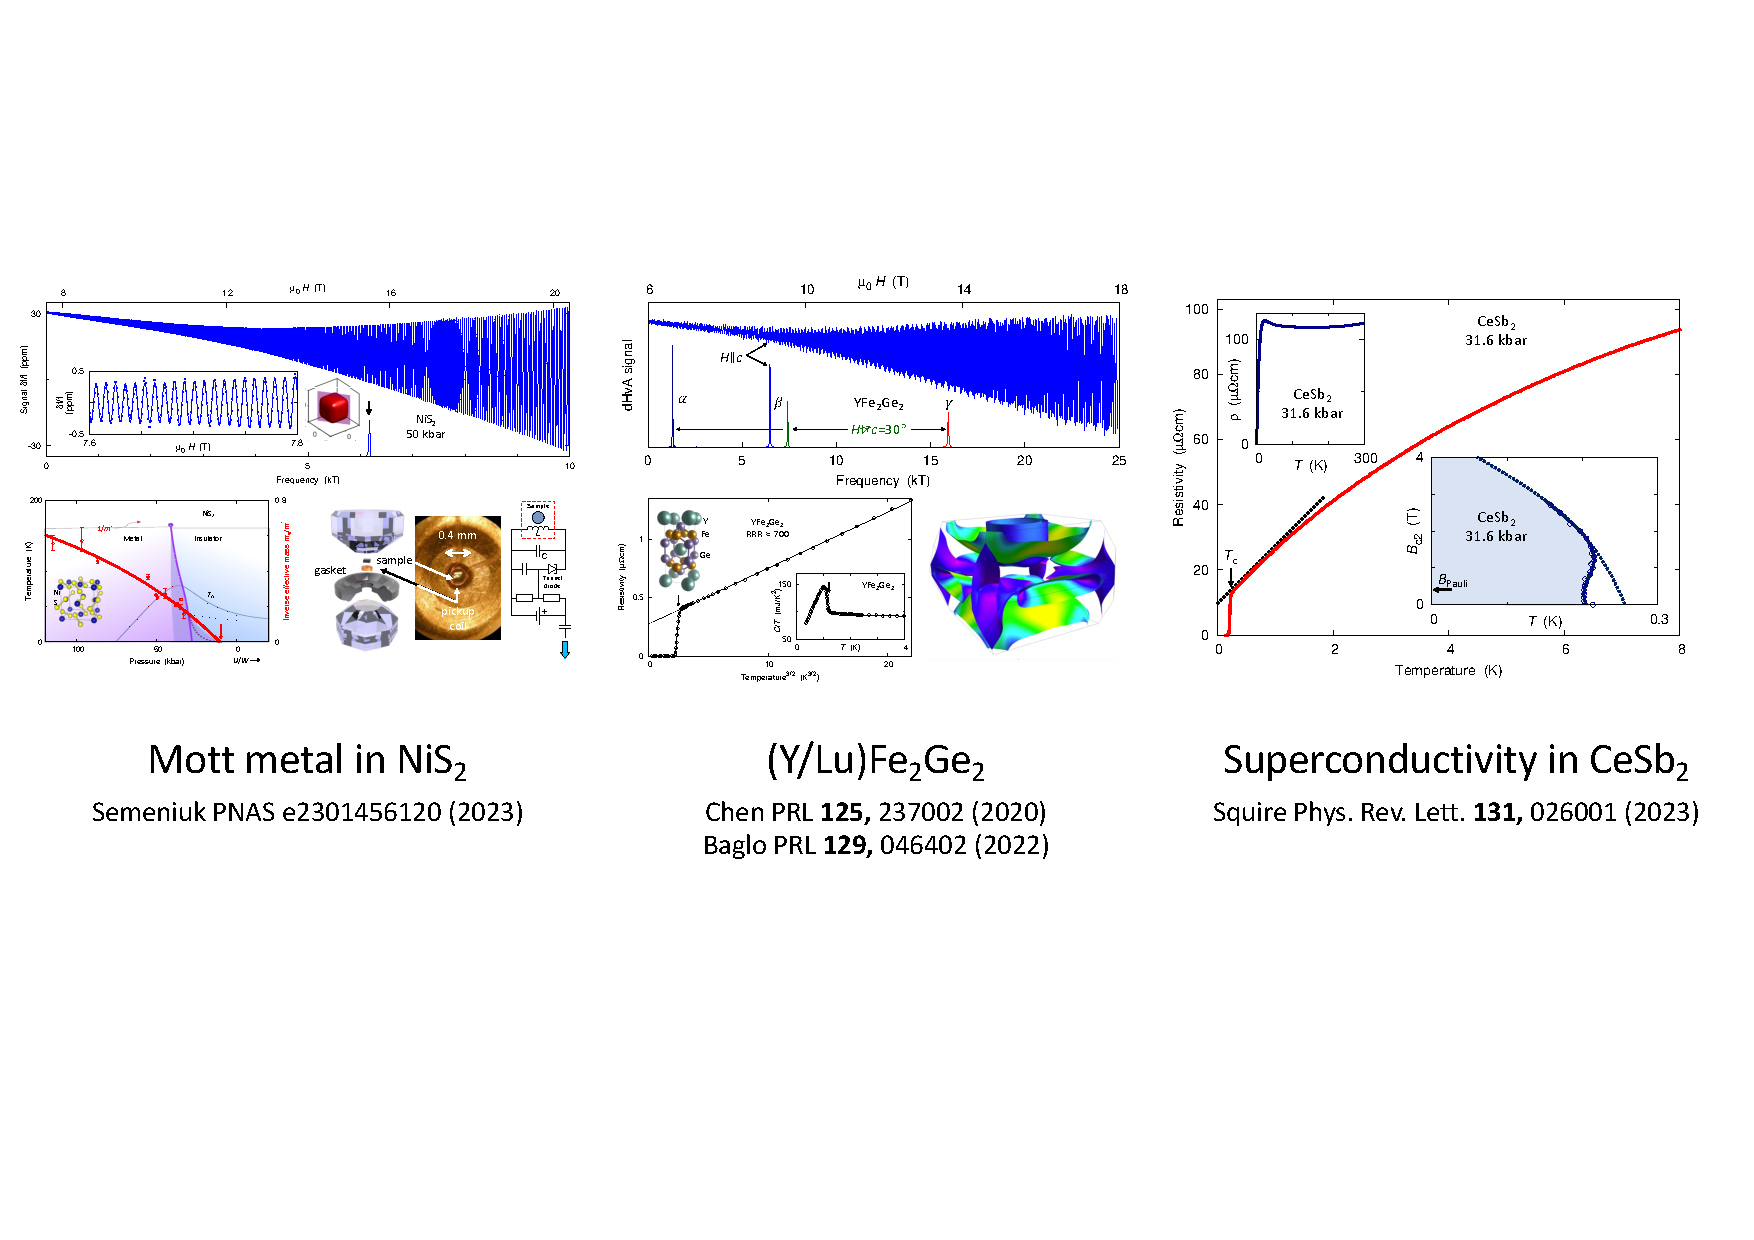
\includegraphics[width=\columnwidth]{IntroPicture5}}

\begin{itemize}
    \item<1-> Present Cambridge Quantum Matter group recent work
    \item<2-> Three classes of correlated electron systems (Mott, Hund's, Kondo)
    \item<3-> Baseline mass enhancement vs. quantum critical point
\end{itemize}
\setbeamercovered{transparent}
\end{emptyframe}
\loadgeometry{beamergeo}



%%% Local Variables: 
%%% mode: latex
%%% TeX-master: "GroTalk.ho"
%%% End: 
